\chapter{序論}
\label{chap:introduction}

\section{背景}
\label{section:background}
高齢化社会の中でひとり暮らしの高齢者が多くなっている。
その中でも糖尿病を患っている人は、他人の監視の目もなく自分で薬物療法などによって治療を行っている。
一人暮らしの中薬の用法容量を守って摂取していくためには習慣化が必須で、最初は特に継続していくのが難しい。

\subsection{糖尿病について}
\label{subsection:diabetes}

糖尿病とは、膵臓から分泌されるインスリンが十分に働かない、もしくは十分に分泌されないことによって、血液中を流れるブドウ糖(血糖)が増えてしまう病気である。\cite{diabetes}
インスリンは元来、血糖を一定の範囲に抑える働きを担っており、これが不足してしまうことは身体機能として異常をきたしていることになる。
血糖値が高い状態が何年も続くことで血管が傷つき、それによる合併症(心臓病、失明、腎不全、足の切断)に繋がる可能性もある。

糖尿病は1型と2型があること、そしてそのその原因と治療法についてここで述べる。

現在の日本において、糖尿病患者の数は実に〇〇人とされ、治療を必要とする人間が多く存在する。
糖尿病は適度な運動を定期的に行っていなかったり、食生活が偏っていることが理由としてあげられる。(ここで糖尿病が上昇傾向にある理由のリファレンスをつける。)

\begin{figure}[htbp]
  \caption{近年における糖尿病患者数の推移(文献\cite{diabetes_statistics}より引用)}
  \label{fig:diabetes_total_number}
  \begin{center}
    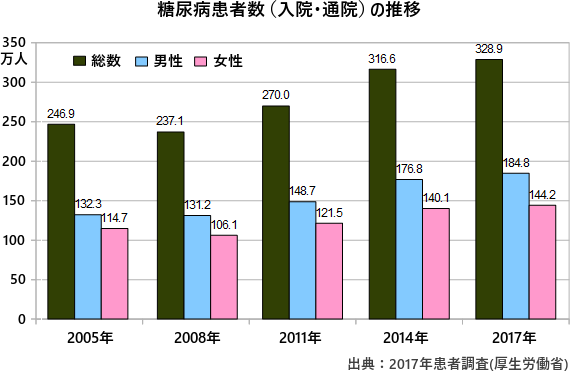
\includegraphics[bb=0 0 900 400,width=25cm]{assets/diabetes_total_number.png}
  \end{center}
\end{figure}

図\ref{fig:diabetes_total_number}は、国勢調査で実際に観測された糖尿病患者数を表している。横軸が左から右へ〇〇年、〇〇年となっていることから、この調査は3年に1度行われていることが見て取れ、
その糖尿病患者数は、〇〇年から毎回上昇していることがわかる。

糖尿病の治療方法としては、運動療法、食事療法、薬物療法が挙げられるが、厚生労働省も掲げる通り、「1に運動2に食事、最後に薬」と言われている。
本論文では、様々ある治療方法の中でも、薬物療法に焦点を絞ってその課題に注目した。

65歳以上の患者数が最多になっていること。

独居老人はどれくらい?独居老人の中で糖尿病を患っている人は?

\subsubsection{糖尿病におけるインスリン治療について}
\label{subsubsection:insulin_treatment}

インスリン治療は、主に糖尿病1型患者、症状や進行状況によっては2型患者も行う治療方法である。具体的には毎食前3回と就寝前1回の計4回、専用の注射器を使い下腹部に自分で直接インスリンを注入するものだ。これにより食事後に起こる血糖値の上昇を一定に抑え、常に血糖値が高くなってしまう状況を回避している。

\paragraph{インスリン注射の手順}
\label{paragraph:insulin_injection_steps}
インスリンを服薬する際の手順を以下に示す。

\begin{enumerate}
  \item \ref{}に示されているような、インスリンの注射の針を注射器に装着する。
  \item 一度注射器の端のメモリをある程度回転させ、注射器の中の空気を押し出す。
  \item 医師に指示を受けている分摂取できるよう注射器の端をねじり、調整する。
  \item 針を刺す下腹部の表面をを消毒し、注射器を刺し、注射器の反対側の端を親指でゆっくり押していく。
  \item 押し切って5秒ほど静止したのち、ゆっくりと針を抜く。
\end{enumerate}


\subsection{一般的な薬物療法について}
\label{subsection:drug_treatment}

ここから一般的な薬物療法に関する課題点の背景を述べる。

一般に、医者から処方された薬を、用法要領を守って服薬し続けることが難しいというアンケート調査結果が図\ref{fig:forget_medicine_number}に示されている。

\begin{figure}[htbp]
  \caption{処方薬の飲み残しに関する意識・実際調査の結果(文献\cite{drug_treatment_investivation}より引用)}
  \label{fig:forget_medicine_number}
  \begin{center}
    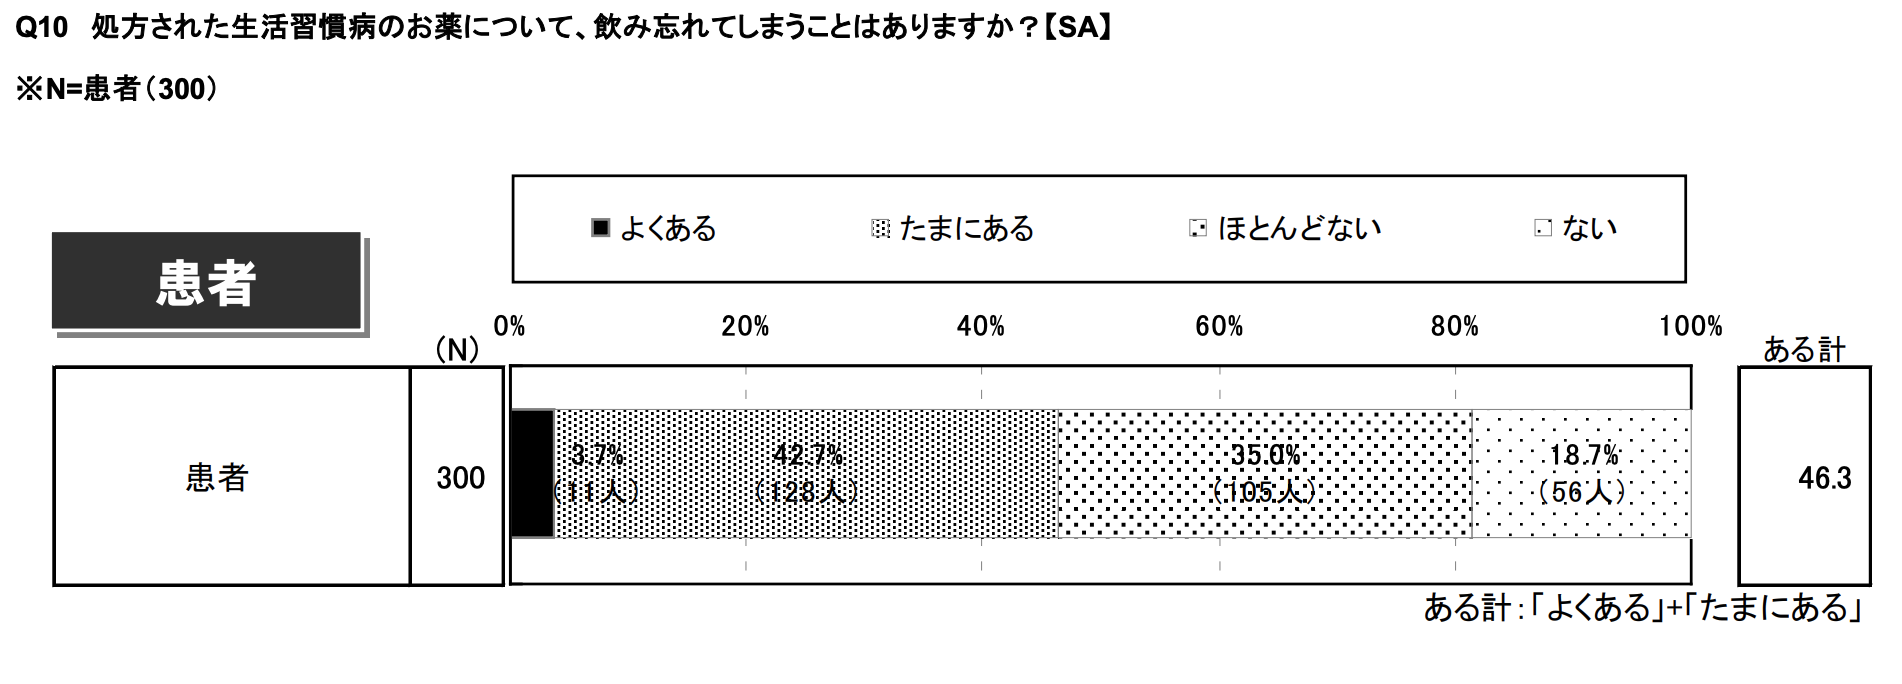
\includegraphics[bb=0 0 1000 400,width=15cm]{assets/forget_medicine_number.png}
  \end{center}
\end{figure}

実際に図\ref{fig:forget_medicine_number}のアンケート結果を見てみると、○%ほどの人が処方された薬を服薬し忘れる傾向があることがわかる。また、この調査は高血圧、高脂血症、糖尿病のいづれかで現在通院中の上、処方薬を使用している生活習慣病の患者を対象にしている\cite{drug_treatment_investigation}ため、本研究で対象としている糖尿病患者も含まれており、薬物治療において服用し忘れが起こる可能性を示唆している。
先ほども\ref{subsection:diabetes}で述べたように、一般的な糖尿病治療の薬の服薬タイミングは厳密に決まっており、毎食前3回と睡眠前1回、インスリンを直接下腹あたりに直接注射することで服用が完了するが、これを忘れると血糖値が上昇したままになってしまうので、糖尿病患者にとってインスリン摂取を忘れることは避けたいものである。

\subsection{問題意識・対象}

どんな人を対象とするのか、どんな食事内容なのか詳細に書く。

\section{本研究で解決したい問題}
\label{section:problem}

本論文では、食前のインスリン注射を服用し忘れてしまい、さらにそれに気づくことができない、という現行の糖尿病治療の課題点に着目した。
現在の治療方法では、患者自身の自己管理能力や、その周りの監視の目に依存してしまっている。
結果として、もし服用を忘れたとしても、それに気づくことなく生活してしまった場合、体調悪化、最悪の場合には合併症を引き起こす可能性もある。
万が一、服用を忘れてしまった場合は、担当医に連絡を取り、状況を説明、そして適切な対処を行うのが一般的である。

\section{目的}
\label{section:purpose}

本研究は、食事前にインスリン注射を服用し忘れたことを治療患者に知らせることを目的としている。
インスリン注射の服用忘れ帽子に関しては、タイマーで時限式に知らせるデバイスがプロダクトとして存在しているが、実際の食事時間が日々異なる可能性を考えると、食事前に服用を行わなければいけない患者にとっての解決策にはならない。
また、食事の検知にはカメラ映像と画像認識技術を使用した研究があるが、被験者にとって常に撮影されているという煩わしさは、実際の導入を考えると現実的ではない。
他にも、顎や腕に直接装着する形のウェアラブルデバイスを用いた食事検知の研究がなされているが、こちらも常に体に装着しておかなければならないことは同じく煩わしさに繋がる。
一方で、本研究では、画像もウェアラブルデバイスも使用せず、食事検知を行うため、以上のような煩わしさはない。

\section{本論文の構成}
\label{section:structure}
本論文における以降の構成は次の通りである。
\ref{chap:related_works}章では、本論文に関連する研究やプロダクトを紹介し、それぞれの特徴とそれらと本研究との差異を示す。
インスリンデバイス、加速度による行動検知、そして食事開始の検知と、幅広く関連研究を挙げている。
\ref{chap:design}章では、加速度センサーによる食事検知とインスリンデバイスによるインスリン摂取忘れを通知するためのシステムの設計について述べる。
\ref{chap:implementation}章では、\ref{chap:design}章で述べた内容の実装に用いたライブラリや実モジュールに言及しながら詳細な実装内容について述べる。
\ref{chap:evaluation}章では、\ref{chap:implementation}章で実装したインスリン摂取忘れ通知システムの評価を行い、その結果について考察する。
\ref{chap:conclusion}章では、本論文のまとめと今後の展望について述べる。
